\documentclass[a4paper, 10pt, ]{article}

\usepackage[slovak]{babel}

% ------------------------------

\usepackage[utf8]{inputenc}
\usepackage[T1]{fontenc}

\usepackage[left=4cm,
            right=4cm,
            top=2.1cm,
            bottom=2.6cm,
            footskip=7.5mm,
            twoside,
            marginparwidth=3.0cm,
            %showframe,
            ]{geometry}

\usepackage{graphicx}
\usepackage[dvipsnames]{xcolor}
% https://en.wikibooks.org/wiki/LaTeX/Colors

% ------------------------------

\usepackage{lmodern}

\usepackage[tt={oldstyle=false,proportional=true,monowidth}]{cfr-lm}
% https://mirror.szerverem.hu/ctan/fonts/cfr-lm/doc/cfr-lm.pdf

% ------------------------------

\usepackage{amsmath}
\usepackage{amssymb}
\usepackage{amsthm}

\usepackage{booktabs}
\usepackage{multirow}
\usepackage{array}
\usepackage{dcolumn}

\usepackage{natbib}

% ------------------------------

\hyphenpenalty=6000
\tolerance=1000

\def\naT{\mathsf{T}}

% ------------------------------

\makeatletter

    \def\@seccntformat#1{\protect\makebox[0pt][r]{\csname the#1\endcsname\hspace{4mm}}}

    \def\cleardoublepage{\clearpage\if@twoside \ifodd\c@page\else
    \hbox{}
    \vspace*{\fill}
    \begin{center}
    \phantom{}
    \end{center}
    \vspace{\fill}
    \thispagestyle{empty}
    \newpage
    \if@twocolumn\hbox{}\newpage\fi\fi\fi}

    \newcommand\figcaption{\def\@captype{figure}\caption}
    \newcommand\tabcaption{\def\@captype{table}\caption}

\makeatother

% ------------------------------

\usepackage{fancyhdr}
\fancypagestyle{plain}{%
\fancyhf{} % clear all header and footer fields
% \fancyfoot[C]{\sffamily {\bfseries \thepage}\ | {\scriptsize\oznacenieCasti}}
\fancyfoot[C]{\sffamily {\bfseries \thepage}{\color{Gray}\scriptsize$\,$z$\,$\pageref{LastPage}}\ | 
\includegraphics[height=5pt]{../../COMMONFILES/KUT_logo_v0.1.pdf}{\scriptsize\KUTporadoveCislo}}
\renewcommand{\headrulewidth}{0pt}
\renewcommand{\footrulewidth}{0pt}}
\pagestyle{plain}

% ------------------------------

\usepackage{titlesec}
\titleformat{\paragraph}[hang]{\sffamily  \bfseries}{}{0pt}{}
\titlespacing*{\paragraph}{0mm}{3mm}{1mm}
\titlespacing*{\subparagraph}{0mm}{3mm}{1mm}

\titleformat*{\section}{\sffamily\Large\bfseries}
\titleformat*{\subsection}{\sffamily\large\bfseries}
\titleformat*{\subsubsection}{\sffamily\normalsize\bfseries}


% ------------------------------

\PassOptionsToPackage{hyphens}{url}
\usepackage[pdfauthor={},
            pdftitle={},
            pdfsubject={},
            pdfkeywords={},
            % hidelinks,
            colorlinks=false,
            breaklinks,
            ]{hyperref}


% ------------------------------

\graphicspath{%
{../fig_standalone/}%
{../../PY/fig/}%
{../../ML/fig/}%
{./fig/}%
}

% ------------------------------

\usepackage{enumitem}

\usepackage{lettrine}

% ------------------------------

\usepackage{lastpage}

\usepackage{microtype}

% ------------------------------

\usepackage{algorithm}
\usepackage[noend]{algpseudocode}
\makeatletter
\renewcommand{\ALG@name}{Algoritmus}
\makeatother
\usepackage{amsmath}
\usepackage{bbold}
\usepackage{calc}
\usepackage{dsfont}
\usepackage{mathtools}
\usepackage{tabto}


\newcommand{\mr}[1]{\mathrm{#1}}
\newcommand{\bs}[1]{\boldsymbol{#1}}
\newcommand{\bm}[1]{\mathbf{#1}}

\newcommand{\diff}[2]{\frac{\Delta #1}{\Delta #2}}
\newcommand{\der}[2]{\frac{d #1}{d #2}}
\newcommand{\parder}[2]{\frac{\partial #1}{\partial #2}}

\newcommand{\argmax}[0]{\mr{argmax}}
\newcommand{\diag}[0]{\mr{diag}}
\newcommand{\rank}[0]{\mr{rank}}
\newcommand{\trace}[0]{\mr{tr}}

\renewcommand{\Re}{\mr{Re}}
\renewcommand{\Im}{\mr{Im}}


\theoremstyle{definition}
\newtheorem{definition}{Definícia}[section]
\newtheorem{theorem}{Veta}[section]
\newtheorem{lemma}[theorem]{Lemma}
\newtheorem{example}{Príklad}[section]
\renewcommand*{\proofname}{Dôkaz}

% ------------------------------


% -----------------------------------------------------------------------------

\def\oznacenieCelku{Kolekcia učebných textov}

% -----------------------------------------------------------------------------


\def\KUTporadoveCislo{017}

% \def\oznacenieVerzie{v0.9}
\def\oznacenieVerzie{\phantom{v1.0}}

\def\mesiacRok{október 2025}

\def\authorslabel{MT}






% -----------------------------------------------------------------------------

\begin{document}

% -----------------------------------------------------------------------------
% Uvodny nadpis

\noindent
\parbox[t][18mm][c]{0.3\textwidth}{%
\raisebox{-0.9\height}{%
\phantom{.}
\includegraphics[height=18mm]{./COMMONFILES/URKFEIlogo.pdf}%
}%
}%
\parbox[t][18mm][c]{0.7\textwidth}{%
\raggedleft

\sffamily
\fontsize{16pt}{18pt}
\fontseries{sbc}
\selectfont

\noindent
\textcolor[rgb]{0.75, 0.75, 0.75}{\textls[25]{\oznacenieCelku}}
}%

\noindent
\parbox[t][16mm][b]{0.5\textwidth}{%
\raggedright

\color{Gray}
\sffamily

\fontsize{12pt}{12pt}
\selectfont
\mesiacRok

\fontsize{6pt}{10pt}
\selectfont
\href{https://github.com/OkoliePracovnehoBodu/KUT}{github.com/OkoliePracovnehoBodu/KUT}

\fontsize{8pt}{10pt}
\selectfont
\authorslabel




}%
\parbox[t][16mm][b]{0.5\textwidth}{%
\raggedleft

\sffamily

\fontsize{6pt}{6pt}
\selectfont

\textcolor[rgb]{0.68, 0.68, 0.68}{\oznacenieVerzie}


\fontsize{14pt}{14pt}
\selectfont

\bfseries


\includegraphics[height=12pt]{./COMMONFILES/KUT_logo_v0.1.pdf}%
{%
\textls[-50]{\KUTporadoveCislo}
}%
}%

% -----------------------------------------------------------------------------




\vspace{6mm}

% ---------------------------------------------
\sffamily
\bfseries
\fontsize{18pt}{21pt}
\selectfont

\begin{flushleft}
    Laboratórne zariadenie TS:\\ softvér pre začiatok
\end{flushleft}

\bigskip

% -----------------------------------------------------------------------------
\normalsize
\normalfont
% -----------------------------------------------------------------------------

\lstset{style=mystyle}










\noindent
\lettrine[lines=1, nindent=1pt, loversize=0.0]{T}{ext} 
uvádza softvér pre uľahčenie začiatku práce s laboratórnym zariadením TS (skratka od \emph{tepelný systém}). 



\section{Úvodné poznámky}





Nasledujúce informácie nadväzujú na opis laboratórneho zariadenia TS a aktuálneho stavu Laboratória kybernetiky uvedený v~dokumentoch:

\medskip

\noindent
\begin{tabular*}{\textwidth}{ @{} >{\sffamily}p{2.0cm} @{\extracolsep{\fill}} p{11cm}<{\raggedright}}

    \href{run:../../KUT_items/KUT015/TeX/KUT015.pdf}{KUT015} & \href{run:../../KUT_items/KUT015/TeX/KUT015.pdf}{Laboratórne zariadenie TS: orientačný prehľad} \\ \addlinespace[3pt]  

    \href{run:../../KUT_items/KUT013/TeX/KUT013.pdf}{KUT013} & \href{run:../../KUT_items/KUT013/TeX/KUT013.pdf}{Laboratórium kybernetiky: zoznam laboratórnych zariadení} \\ \addlinespace[3pt]  

\end{tabular*}

\medskip



\paragraph{MATLAB - Simulink schémy}

Softvérom tu uvedením sú  MATLAB - Simulink schémy (modely) s nakonfigurovanými blokmi prepájajúcimi prostredie Simulink so zariadením TS prostredníctvom meracej karty. 

V laboratóriu je niekoľko zariadení TS a každé je pripojené ku konkrétnej počítačovej zostave. Ku každému zariadeniu prislúcha zodpovedajúca Simulink schéma. Všetky Simulink schémy sú uložené v adresári \texttt{ML} prislúchajúcom k tomuto \textsf{KUT}:

\noindent
% latex-dirtree-gen --ignore TeX,PY,SVG  ./

\dirtree{%
 .1 .
 .2 ML.
 .3 fig.
 .4 TS01\_start.pdf.
 .4 TS01\_start\_TS.pdf.
 .3 TS01\_start.slx.
 .3 TS04\_start.slx.
 .3 TS05\_start.slx.
}







% \textl{01}

\section{Softvér pre jednotlivé zariadenia}


\subsection{Zariadenie TS01, schéma \texttt{TS01\_start.slx}}

Zariadenie \textsf{TS\textl{01}} je pripojené k počítačovej zostave \textsf{LK\textl{31}}. Zodpovedajúca Simulink schéma je \texttt{TS01\_start.slx}. 

Schéma je zobrazená na obr. \ref{TS01_start}. Blok \textl{TS01} predstavuje samotné laboratórne zariadenie. Vstupujúce a vystupujúce signály označené ako \textl{IN1}, \textl{IN2}, \textl{OUT1} a~\textl{OUT2} zodpovedajú signálom opísaným v dokumente \textsf{KUT015}. Príslušnosť signálov k~jednotlivým komponentom zariadenia je tu tiež znázornená na fotografii na obr. \ref{TS_sch3_foto}.

Vnútorné zapojenie bloku \textl{TS01} pre túto schému je zobrazené na obr. \ref{TS01_start_TS} a je dané konkrétnym káblom, prostredníctvom ktorého je zariadenie pripojené k~meracej karte. Rozloženie kontaktov (pinov) v oboch konektoroch kábla sa vo všeobecnosti môže líšiť.

\noindent
\vbox{%

    \makebox[\textwidth][c]{%
	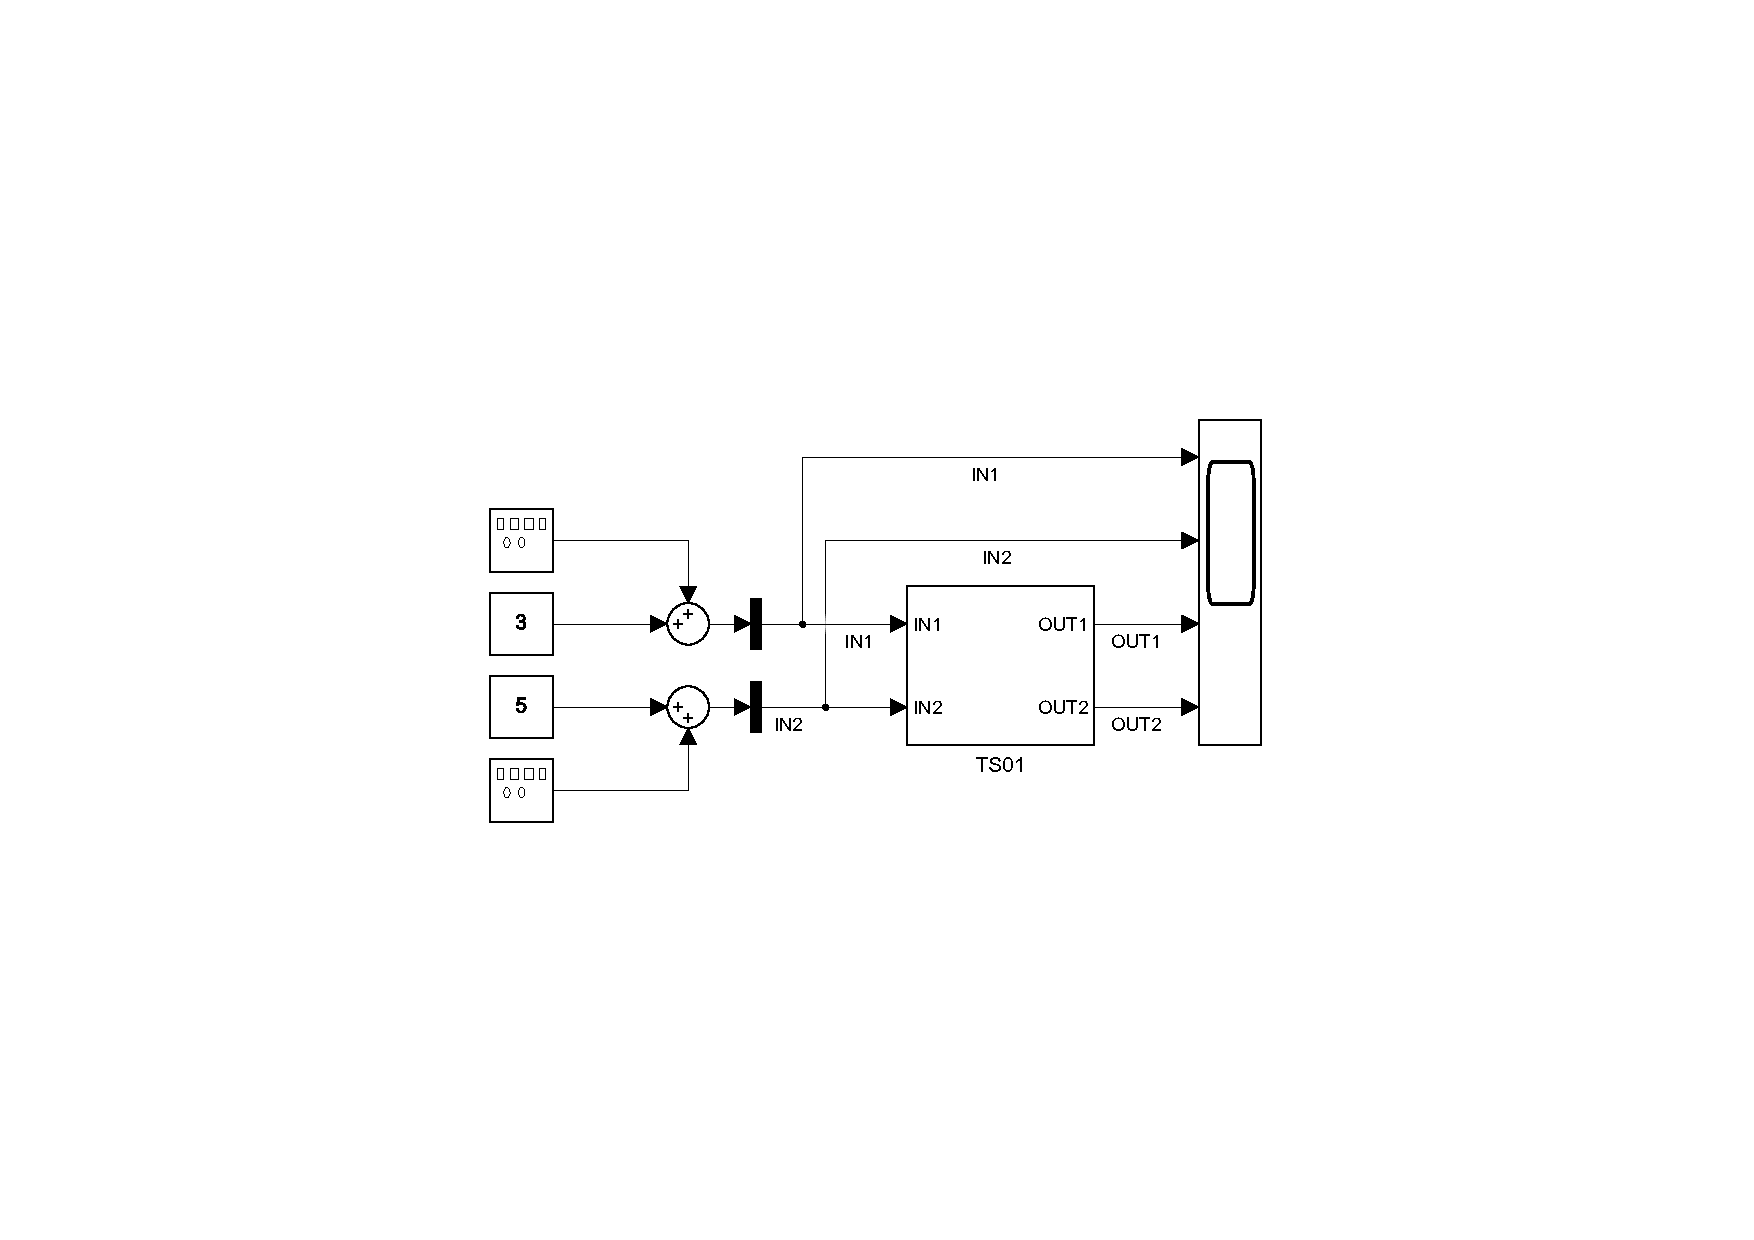
\includegraphics[trim=0mm 68mm 0mm 71mm, clip, scale=0.75]{TS01_start.pdf}
	}

    \vspace{-5mm}

	\figcaption{Simulačná schéma }
	\label{TS01_start}

}%vbox

\smallskip

\noindent
\vbox{%

    \makebox[\textwidth][c]{%
    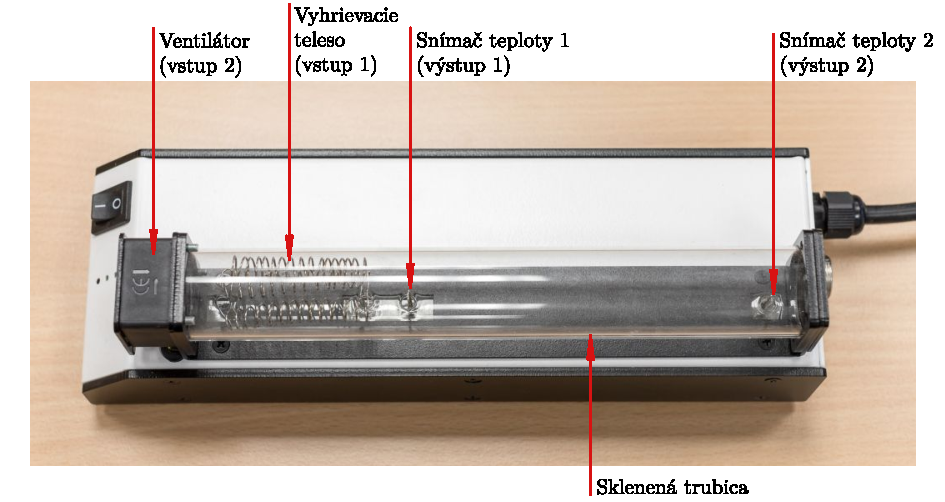
\includegraphics{TS_sch3_foto.pdf}
    }

    \vspace{-3mm}

    \figcaption{ 
        Pohľad zhora na zariadenie TS s vyznačením jednotlivých komponentov. 
    }
    \label{TS_sch3_foto}
}%vbox



\smallskip



\noindent
\vbox{%

    \makebox[\textwidth][c]{%
	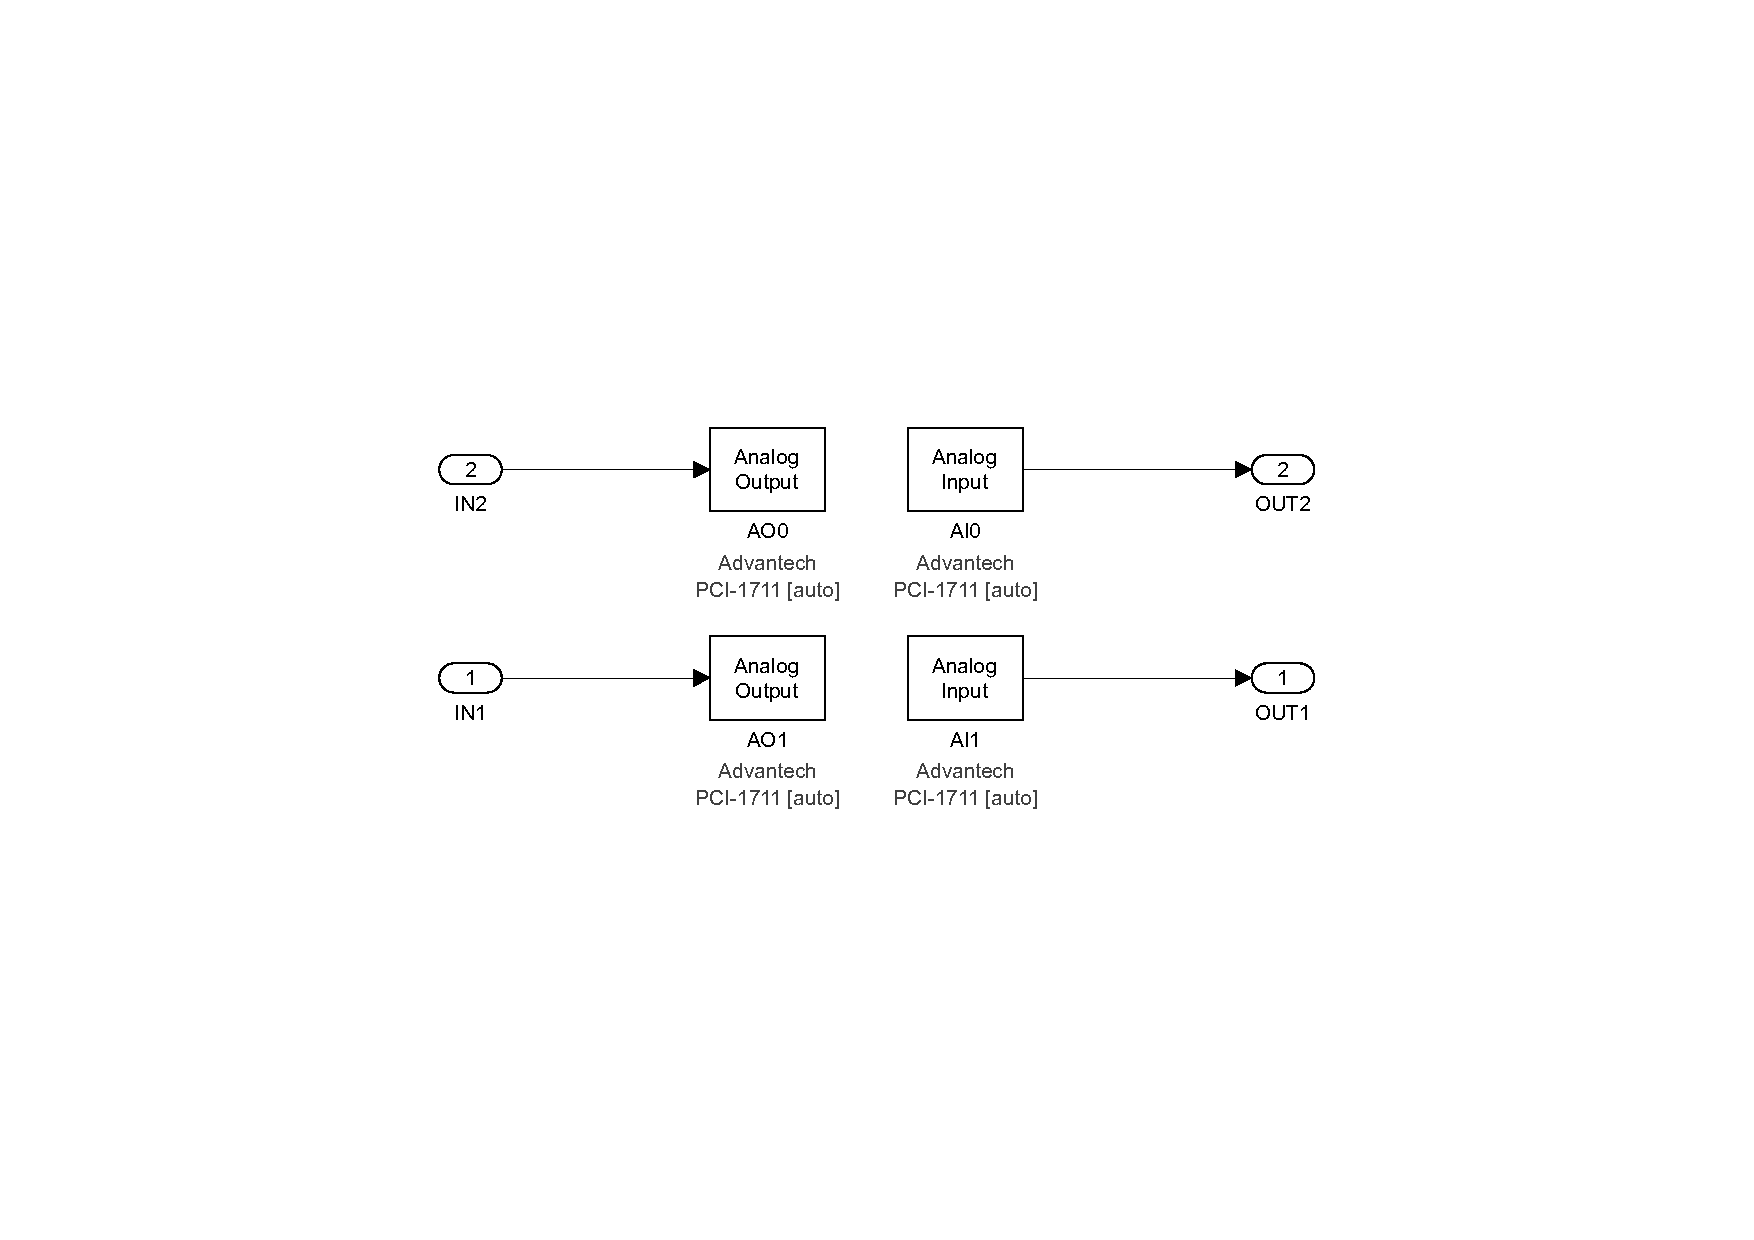
\includegraphics[trim=0mm 67mm 0mm 71mm, clip, scale=0.7]{TS01_start_TS.pdf}
	}

    \vspace{-5mm}

	\figcaption{Prepojenie signálov schémy \texttt{TS01\_start.slx} na analógové vstupy a výstupy meracej karty.  AO$0$ a AO$1$ sú analógové výstupy meracej karty a~AI$0$, AI$1$ sú analógové vstupy meracej karty.
    }
	\label{TS01_start_TS}

}%vbox



\subsection{Zariadenie TS04, schéma \texttt{TS04\_start.slx}}

Zariadenie \textsf{TS\textl{04}} je pripojené k počítačovej zostave \textsf{LK\textl{23}}. Zodpovedajúca Simulink schéma je \texttt{TS04\_start.slx}. Opis schémy je analogický ako v predchádzajúcej časti.


\subsection{Zariadenie TS05, schéma \texttt{TS05\_start.slx}}

Zariadenie \textsf{TS\textl{05}} je pripojené k počítačovej zostave \textsf{LK\textl{32}}. Zodpovedajúca Simulink schéma je \texttt{TS05\_start.slx}. Opis schémy je analogický ako v predchádzajúcej časti.








% -----------------------------------------------------------------------------

\end{document}

% -----------------------------------------------------------------------------